\newcommand{\nom}{Porte conteneur}
\newcommand{\sequence}{03}
\newcommand{\num}{04}
\newcommand{\type}{TD}
\newcommand{\descrip}{Résolution d'un problème en utilisant des méthodes algorithmiques}
\newcommand{\competences}{Alt-C3: Concevoir un algorithme répondant à un problème précisément posé}
\documentclass[10pt,a4paper]{article}
  \usepackage[french]{babel}
  \usepackage[utf8]{inputenc}
  \usepackage[T1]{fontenc}
  \usepackage{xcolor}
  \usepackage[]{graphicx}
  \usepackage{makeidx}
  \usepackage{textcomp}
  \usepackage{amsmath}
  \usepackage{amssymb}
  \usepackage{stmaryrd}
  \usepackage{fancyhdr}
  \usepackage{lettrine}
  \usepackage{calc}
  \usepackage{boxedminipage}
  \usepackage[french,onelanguage, boxruled,linesnumbered]{algorithm2e}
  \usepackage[colorlinks=false,pdftex]{hyperref}
  \usepackage{minted}
  \usepackage{url}
  \usepackage[locale=FR]{siunitx}
  \usepackage{multicol}
  \usepackage{tikz}
  \makeindex

  %\graphicspath{{../Images/}}

%  \renewcommand\listingscaption{Programme}

  %\renewcommand{\thechapter}{\Alph{chapter}}
  \renewcommand{\thesection}{\Roman{section}}
  %\newcommand{\inter}{\vspace{0.5cm}%
  %\noindent }
  %\newcommand{\unite}{\ \textrm}
  \newcommand{\ud}{\mathrm{d}}
  \newcommand{\vect}{\overrightarrow}
  %\newcommand{\ch}{\mathrm{ch}} % cosinus hyperbolique
  %\newcommand{\sh}{\mathrm{sh}} % sinus hyperbolique

  \textwidth 160mm
  \textheight 250mm
  \hoffset=-1.70cm
  \voffset=-1.5cm
  \parindent=0cm

  \pagestyle{fancy}
  \fancyhead[L]{\bfseries {\large PTSI -- Dorian}}
  \fancyhead[C]{\bfseries{{\type} \no \numero}}
  \fancyhead[R]{\bfseries{\large Informatique}}
  \fancyfoot[C]{\thepage}
  \fancyfoot[L]{\footnotesize R. Costadoat, C. Darreye}
  \fancyfoot[R]{\small \today}
  
  \definecolor{bg}{rgb}{0.9,0.9,0.9}
  
  
  % macro Juliette
  
\usepackage{comment}   
\usepackage{amsthm}  
\theoremstyle{definition}
\newtheorem{exercice}{Exercice}
\newtheorem*{rappel}{Rappel}
\newtheorem*{remark}{Remarque}
\newtheorem*{defn}{Définition}
\newtheorem*{ppe}{Propriété}
\newtheorem{solution}{Solution}

\newcounter{num_quest} \setcounter{num_quest}{0}
\newcounter{num_rep} \setcounter{num_rep}{0}
\newcounter{num_cor} \setcounter{num_cor}{0}

\newcommand{\question}[1]{\refstepcounter{num_quest}\par
~\ \\ \parbox[t][][t]{0.15\linewidth}{\textbf{Question \arabic{num_quest}}}\parbox[t][][t]{0.85\linewidth}{#1\label{q\the\value{num_quest}}}\par
~\ \\}

\newcommand{\reponse}[4][1]
{\noindent
\rule{\linewidth}{.5pt}\\
\textbf{Question\ifthenelse{#1>1}{s}{} \multido{}{#1}{%
\refstepcounter{num_rep}\ref{q\the\value{num_rep}} }:} ~\ \\
\ifdef{\public}{#3 ~\ \\ \feuilleDR{#2}}{#4}
}

\newcommand{\cor}
{\refstepcounter{num_cor}
\noindent
\rule{\linewidth}{.5pt}
\textbf{Question \arabic{num_cor}:} \\
}

\usepackage{tikz}
%%\usepackage[a4paper]{geometry}
%\geometry{margin={1cm,1.2cm}}
%\usepackage[francais]{babel}
%\usepackage{nopageno} %pas de numérotation de page
%\pagestyle{plain} %numérotation en bas de page, pas d'entête
%\usepackage{hyperref}
%\usepackage[latin1]{inputenc}

%%%%%%%%%%%%%%%%%%%%%%%%%%%%%%%%%%%%%%%%%%%%%%%%%%%%%%%%%%%%%%%%%%%%%%%%%%%%%%%%%%%%%

\usepackage{amsthm}
\usepackage{amscd}
%\usepackage{mathrsfs}
%\usepackage{amsfonts}
%\usepackage[T1]{fontenc}
%\usepackage{theorem}
\usepackage{lscape}
\usepackage{variations}  % pour faire des tableaux de variations
\usepackage{dsfont}
\usepackage{fancyvrb} % pour mettre Verbatim dans une box

% Pour les figures
\usepackage{subfig}
%\usepackage{calc} % Pour pouvoir donner des formules dans les d�finitions de longueur
%\usepackage{graphicx} % Pour inclure des graphiques 
% Attention : pour inclure des .jpg comme dans l'exemple (ou des .png ou .pdf)
% il faut compiler directement en pdf (commande pdflatex).
% Pour inclure des .eps, il faut compiler avec latex + dvips + ps2pdf.
\usepackage{psfrag}
%\usepackage{color}

%%%%%%%%%%%%%%%%%%%%%%%%%%%%%%%%%%%%%%%%%%%%%%%%%%%%%%%%%%%%%%%%%%%%%%%%%%%%%%%%%%%%%

\theoremstyle{definition}
\newtheorem*{thm}{Théorème}
%\theorembodyfont{\rmfamily}
\newtheorem*{defn}{Définition}
\newtheorem{exercice}{Exercice}
\newtheorem*{problem}{Problème}
\newtheorem*{prop}{Proposition}
\newtheorem*{corollaire}{Corollaire}
\newtheorem*{lemme}{Lemme}
\newtheorem*{remark}{Remarque}
\newtheorem*{notation}{Notation}
\newtheorem*{ex}{Exemple}
\newtheorem*{ppe}{Propriété}
\newtheorem*{meth}{Méthode}
\newtheorem*{rappel}{Rappel}
\newtheorem*{voca}{Vocabulaire}
\setlength{\columnseprule}{0.5pt}


%%%%%%%%%%%%%%%%%%%%%%%%%%%%%%%%%%%%%%%%%%%%%%%%%%%%%%%%%%%%%%%%%%%%%%%%%%%%%%%%%%%%%

\newcommand{\bi}{\bigskip}
\newcommand{\dsp}{\displaystyle}
\newcommand{\noi}{\noindent}
\newcommand{\ov}{\overline}
\newcommand{\dsum}{\displaystyle \sum}
\newcommand{\dprod}{\displaystyle \prod}
\newcommand{\dint}{\displaystyle \int}
\newcommand{\dlim}{\displaystyle \lim}

%%%%%%%%%%%%%%%%%%%%%%%%%%%%%%%%%%%%%%%%%%%%%%%%%%%%%%%%%%%%%%%%%%%%%%%%%%%%%%%%%%%%%


%\newcommand{\pgcd}{\mathrm{pgcd}} % pgcd
%\providecommand{\norm}[1]{\lVert#1\rVert} % norme
%\DeclareMathOperator{\Tan}{Tan}  % espace tangent


\newcommand{\N}{\mathbb{N}}
\newcommand{\Z}{\mathbb{Z}}
\newcommand{\Q}{\mathbb{Q}}
\newcommand{\R}{\mathbb{R}}
\newcommand{\C}{\mathbb{C}}
\newcommand{\K}{\mathbb{K}}
\newcommand{\U}{\mathbb{U}}
\newcommand{\Tr}{\text{Tr}\,}
\newcommand{\pg}{\geqslant}
\newcommand{\pp}{\leqslant}
\newcommand{\bul}{\item[$\bullet$]}
\newcommand{\card}{\text{Card}}
\newcommand{\re}{\text{Re}\;}
\newcommand{\im}{\text{Im}\;}
\newcommand{\Ker}{\text{Ker}\;}
\newcommand{\Vect}{\text{Vect}\;}
\newcommand{\rg}{\text{rg}\;}
\newcommand{\TT}{{}^t\!}
%\newcommand{\sh}{\text{sh}}
%\newcommand{\ch}{\text{ch}}
\newcommand{\Mat}{\text{Mat}}
\usepackage{textcomp}



%%%%%%%%%%%%%%%%%%%%%%%%%%%%%%%%%%%%%%%%%%%%%%%%%%%%%%%%%%%%%%%%%%%%%%%%%%%%%%%%%%%%%%%%%%%%%%%%%%%%%%%%%%%%%%%%%%%%%%%%%%%




\begin{document}

\ifdef{\public}{\excludecomment{solution}}

\begin{center}
{\Large\bf {\type} \no {\numero} -- \descrip}
\end{center}

\SetKw{KwFrom}{de} 

\section{Parcours de graphes}

Dans ce TP, les graphes seront implémentés sous forme de dictionnaires. Par exemple, on considère le graphe suivant : 
\begin{center}
\begin{tikzpicture}[scale=0.7]
\tikzstyle{sommet}=[circle,draw,fill=gray!20]
\draw (1.5,-4.5) node[above] {Graphe \texttt{gr}} ;
\node[sommet] (A) at (-0.5,0.5) {A};
\node[sommet] (B) at (-2,-1.5) {B};
\node[sommet] (C) at (-2,2.5) {C};
\node[sommet] (D) at (1.5,2.5) {D};
\node[sommet] (E) at (1.5,-1.5) {E};
\node[sommet] (F) at (1.5,-3) {F};
\node[sommet] (G) at (3,-1.5) {G};
\node[sommet] (H) at (3.5,1) {H};
\node[sommet] (I) at (4.5,-3) {I};
\node[sommet] (J) at (5,1) {J};
\draw (A) -- (B) -- (C) -- (D) -- (G) -- (H) -- (J);
\draw (B) -- (E) --(F) -- (G) -- (I);
\draw (A) -- (E) ;
\draw (A) -- (D) ;
\end{tikzpicture}
\end{center}
Le dictionnaire qui le représente commence comme : 
\begin{center}
\texttt{gr = \{'A' : ['B' , 'D' , 'E'], 'B' : ['A' , 'C' , 'E'], ...\}}
\end{center}

\begin{exercice}
Écrire le dictionnaire complet associé au graphe \texttt{gr}.
\end{exercice}

\begin{solution}
\texttt{gr=\{'A':['B','D','E'],'B':['A','C','E'],'C':['B','D'],'D':['A','C','G'],}\\
\texttt{'E':['A','B','F'],'F':['E','G'],'G':['D','F','H','I'],'H':['G','J'],'I':['G'],'J':['H']\}}
\end{solution}

\begin{exercice}Parcours en largeur.
\begin{enumerate}
\item Écrire une fonction \texttt{ParcoursLargeur} qui étant donné un graphe et un sommet de ce graphe, réalise un parcours en largeur et retourne la liste des sommets dans l'ordre dans lequel ils ont été explorés.
\item Tester votre fonction sur le graphe donné en exemple. \\
\texttt{ParcoursLargeur(gr,'A')} renvoie \texttt{['A', 'B', 'D', 'E', 'C', 'G', 'F', 'H', 'I', 'J']}.
\item Modifier la fonction \texttt{ParcoursLargeur} afin qu'elle affiche les n\oe uds à explorer à chaque étape.
\item Commenter si cette suite d'élément se comporte en \texttt{pile} ou en \texttt{file}.
\end{enumerate}
\end{exercice}

\begin{solution}~\
\begin{minted}[linenos,frame=lines]{python}
def PL2(gr,s):
    files=[s]
    noeuds_decouverts=[s]
    while len(files)!=0:
        print(files)
        noeud_courant=files[0]
        files=files[1:]
        for voisin in gr[noeud_courant]:
            if voisin not in noeuds_decouverts:
                noeuds_decouverts.append(voisin)
                files.append(voisin)
    return(noeuds_decouverts)    
\end{minted}
Les noeuds entrent par la fin et sortent par l'avant, il s'agit donc d'une file.
\end{solution}


\begin{exercice}Parcours en profondeur.
\begin{enumerate}
\item Écrire une fonction \texttt{ParcoursProfondeur} qui étant donné un graphe et un sommet de ce graphe, réalise un parcours en profondeur et retourne la liste des sommets dans l'ordre dans lequel ils ont été explorés.
\item Tester votre fonction sur le graphe donné en exemple. \\ \texttt{ParcoursProfondeur(gr,'A')} renvoie \texttt{['A', 'E', 'F', 'G', 'I', 'H', 'J', 'D', 'C', 'B']}.
\item Modifier la fonction \texttt{ParcoursProfondeur} afin qu'elle affiche les n\oe uds à explorer à chaque étape.
\item Commenter si cette suite d'élément se comporte en \texttt{pile} ou en \texttt{file}.
\end{enumerate}
\end{exercice}

\begin{solution}~\
\begin{minted}[linenos,frame=lines]{python}
def PP2(gr,s):
    piles=[s]
    noeuds_decouverts=[]
    while len(piles)!=0:
        print(piles)
        noeud_courant=piles[-1]
        piles=piles[:-1]
        for voisin in gr[noeud_courant]:
            if (voisin not in noeuds_decouverts) and (voisin not in piles):
                piles.append(voisin)   
        noeuds_decouverts.append(noeud_courant)
                
    return(noeuds_decouverts)
\end{minted}
Les noeuds entrent par la fin et sortent par la fin, il s'agit donc d'une pile.
\end{solution}


\begin{exercice}Composantes connexes.
\begin{enumerate}
\item Écrire une fonction \texttt{EstConnexe} qui prend un graphe comme argument et renvoie \texttt{True} si le graphe est connexe et \texttt{False} sinon.
Par exemple, pour le graphe précédent, \texttt{EstConnexe(gr)} renvoie \texttt{True}.
\item Écrire une fonction \texttt{NbCompConnexe} qui prend un graphe comme argument et renvoie le nombre de composantes connexes de ce graphe. \\
Par exemple, pour le graphe suivant, la fonction doit renvoyer 3.
\begin{center}
\begin{tikzpicture}[scale=0.5]
\tikzstyle{sommet}=[circle,draw,fill=gray!20]
\draw (1.5,-4.5) node[above] {Graphe à 3 composantes connexes} ;
\node[sommet] (A) at (-0.5,0.5) {A};
\node[sommet] (B) at (-2,-1.5) {B};
\node[sommet] (C) at (-2,2.5) {C};
\node[sommet] (D) at (1.5,2.5) {D};
\node[sommet] (E) at (1.5,-1.5) {E};
\node[sommet] (F) at (3,-3) {F};
\node[sommet] (G) at (5,-1.5) {G};
\node[sommet] (H) at (5.5,1) {H};
\node[sommet] (I) at (8,-3) {I};
\node[sommet] (J) at (8,1) {J};
\draw (A) -- (B) -- (C) -- (D);
\draw (B) -- (E);
\draw (A) -- (E) ;
\draw (A) -- (D) ;
\draw  (G) -- (H) -- (J) -- (I);
\end{tikzpicture}
\end{center}
\end{enumerate}
\end{exercice}

\begin{solution}~\
\begin{minted}[linenos,frame=lines]{python}
def EstConnexe(gr):
    sommet=gr.keys()[0]
    liste=PL(gr,sommet)
    return(len(liste)==len(gr.keys()))


def NbCompConnexe(gr):
    liste_sommets=gr.keys()
    Nb=0
    while len(liste_sommets)!=0:
        Nb=Nb+1
        sommet=liste_sommets[0]
        for voisin in PL(gr,sommet):
            liste_sommets.remove(voisin)
    return(Nb) 
\end{minted}
\end{solution}

\section{Algorithme de Dijkstra}

On considère un graphe connexe pondéré avec des poids positifs. L'objectif est de trouver le chemin entre deux sommets qui minimise la somme des poids rencontrés. 

\begin{center}
\begin{tikzpicture}[scale=1]
\tikzstyle{sommet}=[circle,draw,fill=gray!20]
\tikzstyle{arete}=[midway,fill=white]
\node[sommet] (S0) at ( 90:1.5) {A};
\node[sommet] (S1) at (162:1.5) {B};
\node[sommet] (S2) at (234:1.5) {C};
\node[sommet] (S3) at (306:1.5) {D};
\node[sommet] (S4) at ( 18:1.5) {E};
%\node[fill=white] (h) at (1.58,-1.21) {$h$};
\draw (S0) -- (S1) node[arete] {$1$} 
-- (S2) node[arete] {$5$} 
-- (S3) node[arete] {$2$}
-- (S4) node[arete] {$7$}
-- (S0) node[arete] {$2$};
%\draw (S0) -- (S2) node[arete] {$f$} 
%-- (S4) node[arete] {$g$};
%\draw (S3) to[out=45,in=90] (h) to[out=-90,in=-45] (S3) ;
\end{tikzpicture}
\end{center}

Un tel graphe peut être représenté par un dictionnaire de dictionnaires. Celui ci-dessus commence par :
\begin{center}
\texttt{gr = \{'A' : \{ 'B' : 1 , 'E' : 2  \} , ...\}}
\end{center}

L'algorithme de Dijkstra permet de répondre à ce problème selon le principe suivant :\\
au départ, la distance au sommet $A$ est nulle et toutes les autres distances sont infinies. Le sommet $A$ est alors exploré.\\
A chaque itération : 
\begin{itemize}
\item on découvre les sommets adjacents ;
\item la distance d'un trajet est égale à la somme des poids des arcs ;
\item on choisit le prochain sommet à explorer comme celui qui est à distance minimale du sommet de départ.
\end{itemize}
On s'arrête quand tous les sommets ont été explorés.\\

On applique l'algorithme sur l'exemple précédent pour minimiser la distance entre $A$ et $D$ (on souligne à chaque étape la distance minimale pour choisir le n\oe ud à explorer) :

\begin{center}
\begin{tikzpicture}[scale=1]
\tikzstyle{sommet}=[circle,draw,fill=gray!20]
\tikzstyle{arete}=[midway,fill=white]
\node[sommet] (S0) at ( 90:1.5) {\underline{A}{\tiny0}};
\node[sommet] (S1) at (162:1.5) {B{\tiny$\infty$}};
\node[sommet] (S2) at (234:1.5) {C{\tiny$\infty$}};
\node[sommet] (S3) at (306:1.5) {D{\tiny$\infty$}};
\node[sommet] (S4) at ( 18:1.5) {E{\tiny$\infty$}};
\draw (S0) -- (S1) node[arete] {$1$} 
-- (S2) node[arete] {$5$} 
-- (S3) node[arete] {$2$}
-- (S4) node[arete] {$7$}
-- (S0) node[arete] {$2$};
\end{tikzpicture}\quad 
\begin{tikzpicture}[scale=1]
\tikzstyle{sommet}=[circle,draw,fill=gray!20]
\tikzstyle{arete}=[midway,fill=white]
\node[sommet] (S0) at ( 90:1.5) {\underline{A}{\tiny0}};
\node[sommet] (S1) at (162:1.5) {\underline{B}{\tiny1}};
\node[sommet] (S2) at (234:1.5) {C{\tiny$\infty$}};
\node[sommet] (S3) at (306:1.5) {D{\tiny$\infty$}};
\node[sommet] (S4) at ( 18:1.5) {E{\tiny2}};
\draw (S0) -- (S1) node[arete] {$1$} 
-- (S2) node[arete] {$5$} 
-- (S3) node[arete] {$2$}
-- (S4) node[arete] {$7$}
-- (S0) node[arete] {$2$};
\end{tikzpicture}\quad
\begin{tikzpicture}[scale=1]
\tikzstyle{sommet}=[circle,draw,fill=gray!20]
\tikzstyle{arete}=[midway,fill=white]
\node[sommet] (S0) at ( 90:1.5) {\underline{A}{\tiny0}};
\node[sommet] (S1) at (162:1.5) {\underline{B}{\tiny1}};
\node[sommet] (S2) at (234:1.5) {C{\tiny6}};
\node[sommet] (S3) at (306:1.5) {D{\tiny$\infty$}};
\node[sommet] (S4) at ( 18:1.5) {\underline{E}{\tiny2}};
\draw (S0) -- (S1) node[arete] {$1$} 
-- (S2) node[arete] {$5$} 
-- (S3) node[arete] {$2$}
-- (S4) node[arete] {$7$}
-- (S0) node[arete] {$2$};
\end{tikzpicture}
\end{center}
\begin{center}
\begin{tikzpicture}[scale=1]
\tikzstyle{sommet}=[circle,draw,fill=gray!20]
\tikzstyle{arete}=[midway,fill=white]
\node[sommet] (S0) at ( 90:1.5) {\underline{A}{\tiny0}};
\node[sommet] (S1) at (162:1.5) {\underline{B}{\tiny1}};
\node[sommet] (S2) at (234:1.5) {\underline{C}{\tiny6}};
\node[sommet] (S3) at (306:1.5) {D{\tiny9}};
\node[sommet] (S4) at ( 18:1.5) {\underline{E}{\tiny2}};
\draw (S0) -- (S1) node[arete] {$1$} 
-- (S2) node[arete] {$5$} 
-- (S3) node[arete] {$2$}
-- (S4) node[arete] {$7$}
-- (S0) node[arete] {$2$};
\end{tikzpicture}
\quad
\begin{tikzpicture}[scale=1]
\tikzstyle{sommet}=[circle,draw,fill=gray!20]
\tikzstyle{arete}=[midway,fill=white]
\node[sommet] (S0) at ( 90:1.5) {\underline{A}{\tiny0}};
\node[sommet] (S1) at (162:1.5) {\underline{B}{\tiny1}};
\node[sommet] (S2) at (234:1.5) {\underline{C}{\tiny6}};
\node[sommet] (S3) at (306:1.5) {\underline{D}{\tiny8}};
\node[sommet] (S4) at ( 18:1.5) {\underline{E}{\tiny2}};
\draw (S0) -- (S1) node[arete] {$1$} 
-- (S2) node[arete] {$5$} 
-- (S3) node[arete] {$2$}
-- (S4) node[arete] {$7$}
-- (S0) node[arete] {$2$};
\end{tikzpicture}
\end{center}

%\begin{center}
%\begin{tabular}{|c||c|c|c|c|c|}
%\hline
%noeuds à explorer & à $A$ & à $B$ & à $C$ & à $D$ & à $E$ \\
%\hline
%\hline
%$A$ & \underline{0} & $+\infty$ & $+\infty$ & $+\infty$ & $+\infty$ \\
%\hline
%$B$ & - & \underline{1} & $+\infty$ & $+\infty$ & 2 \\
%\hline
%$E$ & - & - & 6 & $+\infty$ & \underline{2} \\
%\hline
%$C$ & - & - & \underline{6} & 9 & - \\
%\hline
%$D$ & - & - & - & \underline{8} & - \\
%\hline
%\end{tabular}
%\end{center}


\begin{exercice}
Appliquer à la main l'algorithme de Dijkstra au graphe ci-dessous entre les sommets $A$ et~$G$.
\begin{center}
\begin{tikzpicture}[scale=0.7]
\tikzstyle{sommet}=[circle,draw,fill=gray!20]
\tikzstyle{arete}=[midway,fill=white]
\node[sommet] (A) at (1.5,2.5) {A};
\node[sommet] (B) at (-1,0) {B};
\node[sommet] (C) at (1.5,0) {C};
\node[sommet] (D) at (4,0) {D};
\node[sommet] (E) at (-1,-2.5) {E};
\node[sommet] (F) at (1.5,-2.5) {F};
\node[sommet] (G) at (4,-2.5) {G};
\draw (A) -- (B) node[arete] {$5$} 
-- (E) node[arete] {$10$} 
-- (F) node[arete] {$2$} 
-- (G) node[arete] {$8$} ;
\draw (A)-- (C) node[arete] {$10$} 
-- (F) node[arete] {$21$} ;
\draw (A)-- (D) node[arete] {$9$} 
-- (G) node[arete] {$32$} ;
 %  -- (G) -- (H) -- (J);
%\draw (B) -- (E) --(F) -- (G) -- (I);
%\draw (A) -- (E) ;
%\draw (A) -- (D) ;
\end{tikzpicture}
\end{center}
\end{exercice}

\begin{solution}
\begin{center}
\begin{tabular}{|c||c|c|c|c|c|c|c|}
\hline
noeuds à explorer & à $A$ & à $B$ & à $C$ & à $D$ & à $E$ &  à $F$ & à $G$ \\
\hline
\hline
$A$ & \underline{0} & $+\infty$ & $+\infty$ & $+\infty$ & $+\infty$ & $+\infty$ & $+\infty$ \\
\hline
$B$ & - & \underline{5} & 10 & 9 & $+\infty$ & $+\infty$ & $+\infty$ \\
\hline
$D$ & - &- & 10 & \underline{9} & 15 & $+\infty$ & $+\infty$ \\
\hline
$C$ & - &- & \underline{10} & - & 15 & $+\infty$ & 41 \\
\hline
$E$ & - &- & - & - & \underline{15} & 31 & 41 \\
\hline
$F$ & - &- & - & - & - & \underline{17} & 41 \\
\hline
$G$ & - &- & - & - & - & - & 25 \\
\hline
\end{tabular}
\end{center}
Chemin minimal : \texttt{'A'-'B'-'E'-'F'-'G'}
\end{solution}


\begin{exercice}
Dans l'algorithme, à chaque itération, on a besoin de choisir le chemin le plus court parmi ceux déjà explorés. 
Écrire une fonction \texttt{MinDistance} qui à un dictionnaire du type \texttt{\{'A' : 1, 'B' : 4, 'C' : 0\}} renvoie le sommet de poids minimal.
\end{exercice}

\begin{solution}~\
\begin{minted}[linenos,frame=lines]{python}
def MinDistance(sousgr):
    sommet_mini=sousgr.keys()[0]
    mini=sousgr[sommet_mini]
    for sommet in sousgr.keys():
        if sousgr[sommet]<mini:
            mini=sousgr[sommet]
            sommet_mini=sommet
    return(sommet_mini) 
\end{minted}
\end{solution}



\begin{exercice}
Ouvrir le fichier CodeDijkstra.py dans le lequel se trouve la fonction \texttt{Dijkstra} (version récursive), rédigée par Frank Chevrier. Elle prend comme entrée un graphe pondéré (présenté sous forme de dictionnaire) et deux sommets du graphe et renvoie le chemin le plus court. Tester cette fonction sur un graphe pondéré.
\end{exercice}

\begin{solution}

\end{solution}


\section{Application : temps de trajet en métro}

\textit{D'après une idée de Michel Couprie et Gilles Bertrand}

\begin{center}
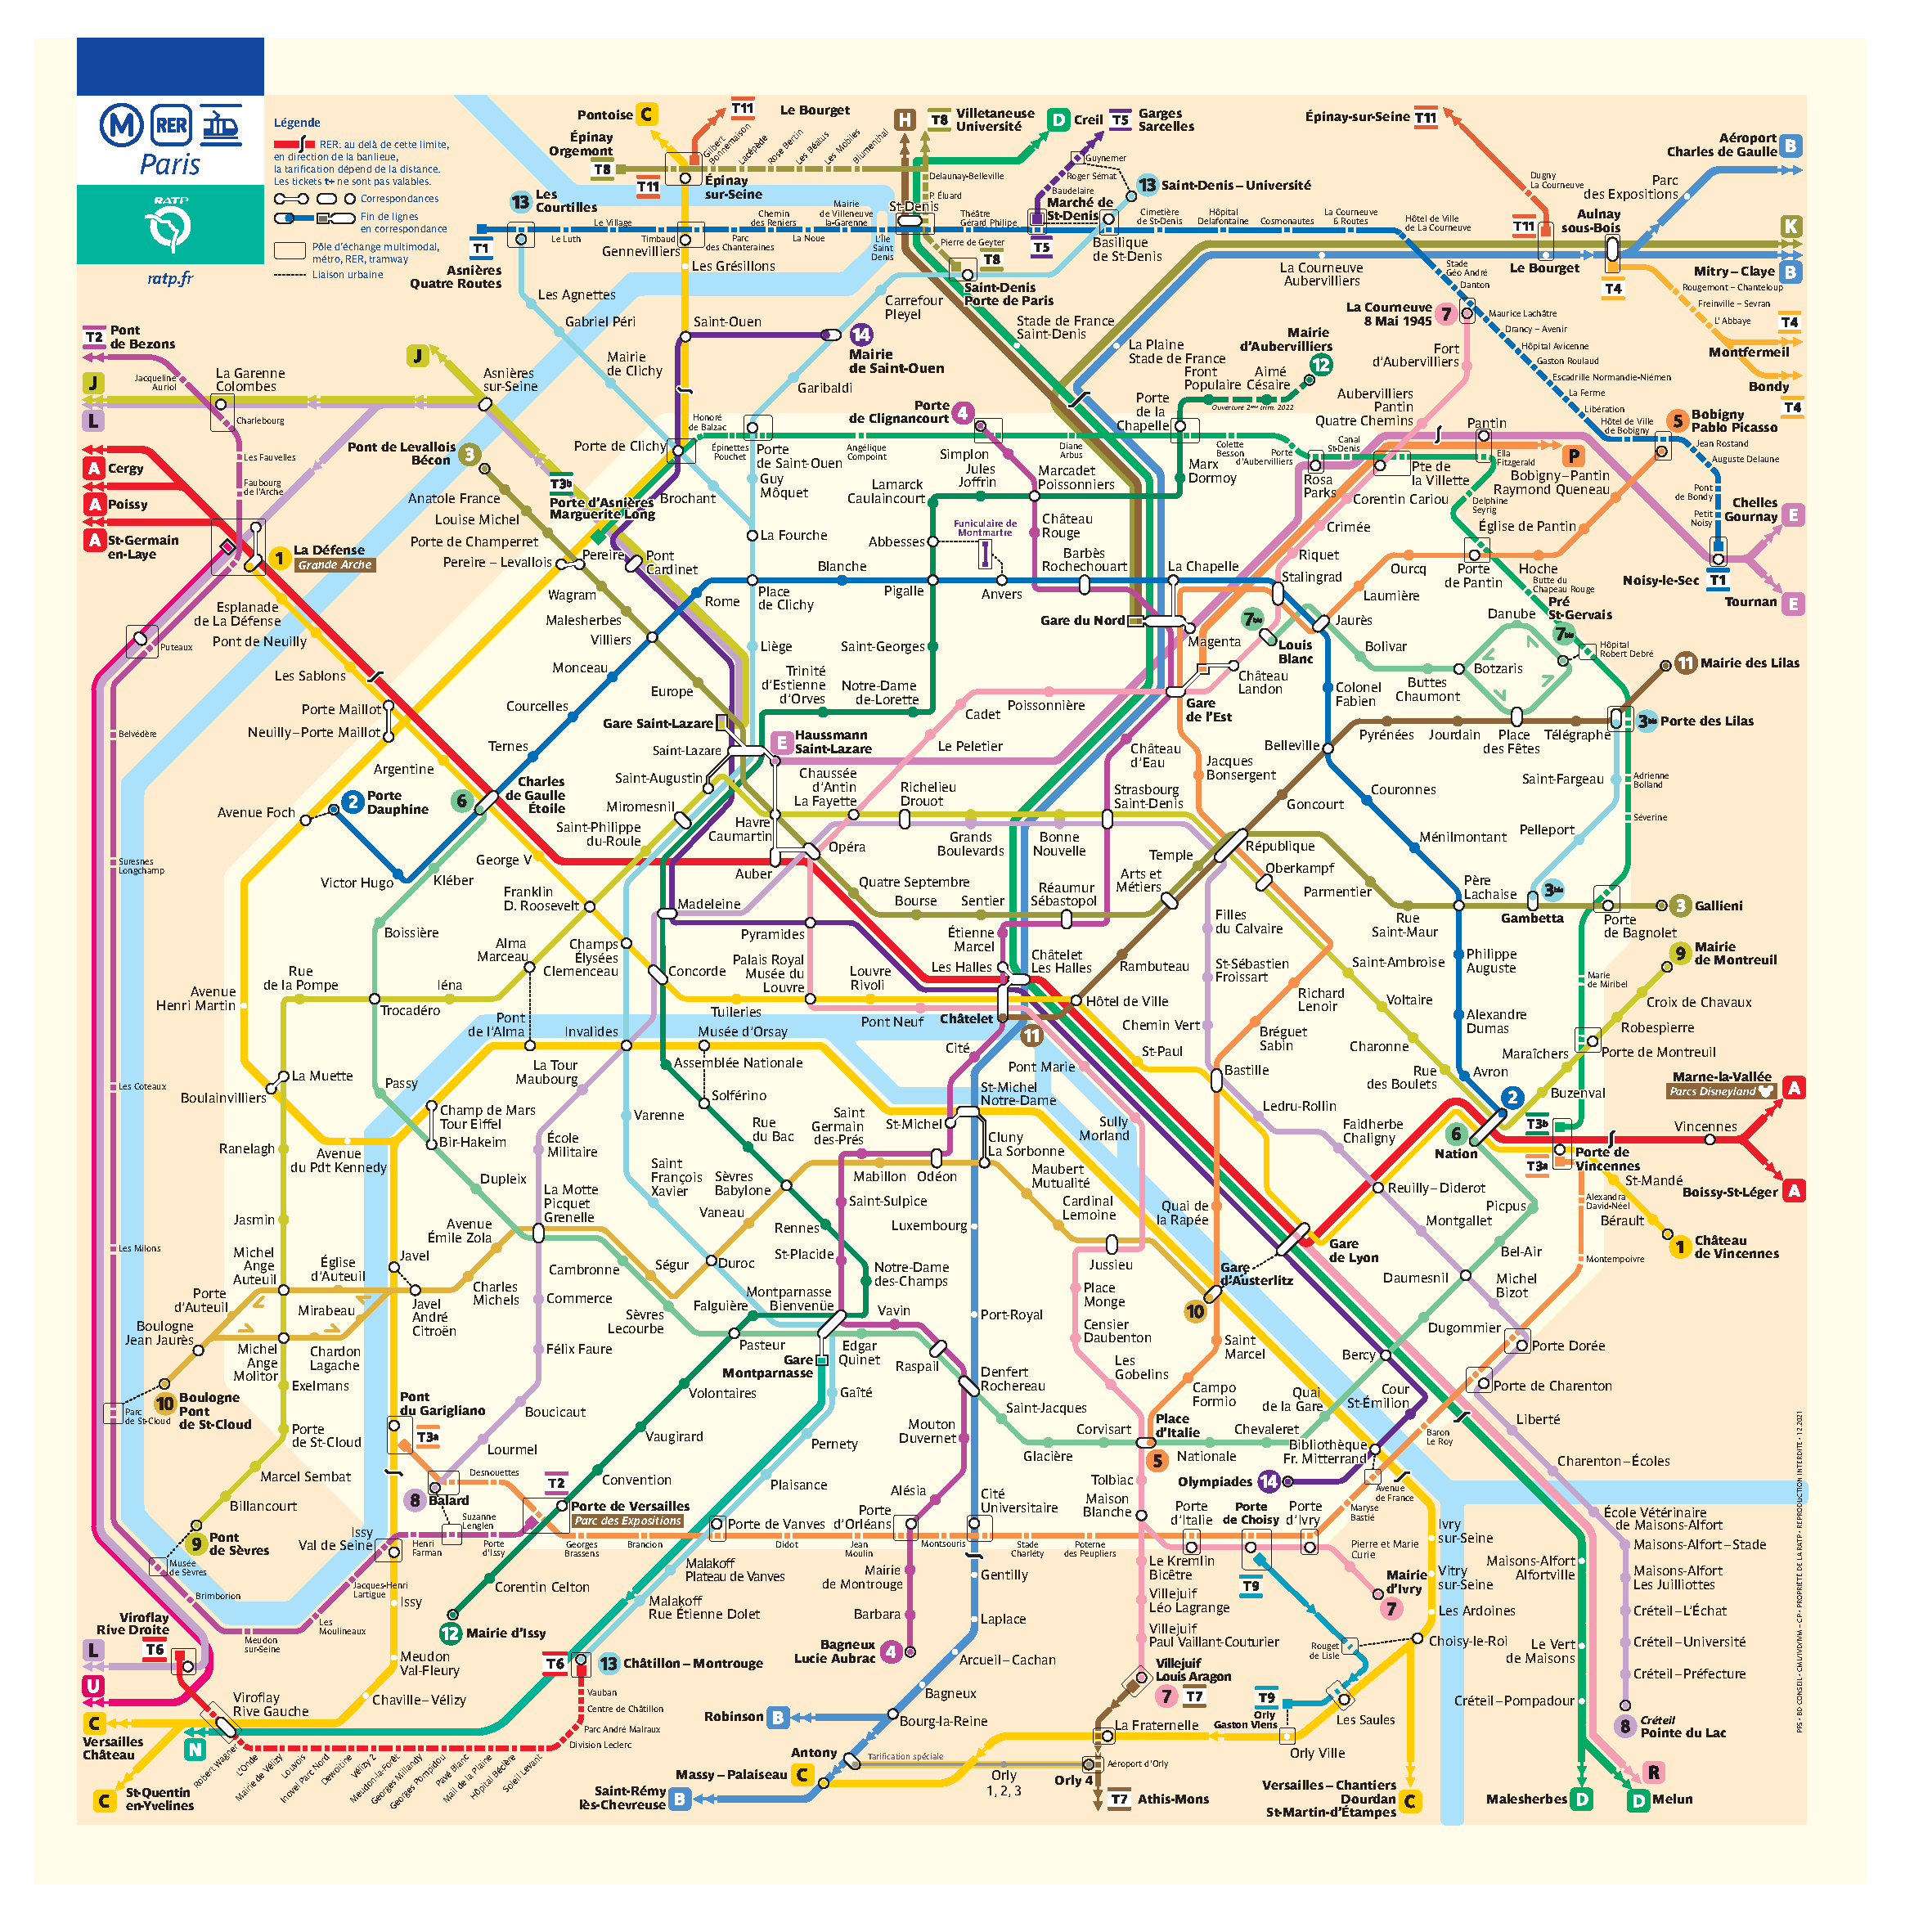
\includegraphics[scale=0.3]{metro/Plan.pdf}
\end{center}
On considère le plan du métro parisien. Chaque sommet correspond à une station pour une ligne. Par exemple, il y a 5 sommets "République". Deux sommets sont reliés par une arête pondérée par le temps de trajet en seconde entre les deux stations. Il existe aussi une arête entre les stations de même nom. Ces arêtes sont toutes pondérées par 120 (autrement dit, on compte 120s pour effecteur une correspondance).

\begin{exercice}
\begin{enumerate}
\item Combien d'arêtes partent du sommet "Croix de Chavaux" ? d'un des sommets "République" ?
\item Expliquer pourquoi le graphe est orienté.
\end{enumerate}
\end{exercice}

\begin{solution}
\begin{enumerate}
\item Deux arêtes partent de "Croix de Chavaux". L'une la relie à 'Mairie de Montreuil', l'autre à 'Robespierre'.\\
Depuis l'un des sommet "République", on a deux arêtes qui partent pour aller aux stations voisines sur la même ligne et on a 4 arêtes qui relient aux autres sommets 'République'.
\item La ligne 7 bis par exemple ne pas pas être parcourue de façon symétrique.
\end{enumerate}
\end{solution}


Dans le fichier data\_nom.csv, on trouve les noms des stations, avec chacune un numéro. Dans le fichier data\_arete.csv, chaque ligne contient trois nombres : le numéro de la station de départ, le numéro de la station d'arrivée, le temps de trajet. 

\begin{exercice}
\begin{enumerate}
\item Importer les deux fichiers sous forme de deux tableaux : le premier tableau aura deux colonnes (entier, chaîne de caractères), le deuxième trois colonnes (entier, entier, flottant).
\item Construire le dictionnaire associé à ce graphe pondéré.
\item Appliquer la fonction \texttt{Dijkstra} à ce graphe, entre deux stations.
\end{enumerate}
\end{exercice}

\begin{solution}~\
\begin{minted}[linenos,frame=lines]{python}
fichier = open("data/data_nom.csv", "r")
fichier2 = open("data/data_arete.csv", "r")

tableau=fichier.read()
tableau2=fichier2.read()

fichier.close()
fichier2.close()

lignes=tableau.split('\n')
nom=[]
for i in lignes[:-1]:
    ligne=i.split(',')
    ligne[0]=int(ligne[0])
    nom.append(ligne)
    
lignes2=tableau2.split('\n')    
arete=[]
for i in lignes2[:-1]:
    ligne=i.split(',' )
    arete.append([int(ligne[0]),int(ligne[1]),float(ligne[2])])
    
dico={}
for i in arete:
    if i[0] not in dico:
        dico[i[0]]={i[1]:i[2]}
    else:
        dico[i[0]][i[1]]=i[2]

Trajet=Dijkstra(dico,88,302)

print(Trajet[0]/60.)
for i in Trajet[1]:
    print(nom[i])
\end{minted}
\end{solution}



\end{document}







L'algorithme suivant va déterminer les distances entre le sommet $A$, et les autres sommets sous la forme d'un dictionnaire. Voici les étapes :\\
\begin{algorithm}[H]
\SetAlgoLined
 \textbf{Initialisation}\;
 Initialiser le dictionnaire \texttt{distance} qui, à chaque sommet du graphe, associe $+\infty$, hormis le sommet initial $A$ qu'on associe à $0$ \;
 Initialiser la liste \texttt{sommets\_a\_explorer} comme une liste contenant tous les sommets \;
 \Tq{\texttt{sommets\_a\_explorer} n'est pas la liste de tous les sommets}{
  n\oe ud\_courant $\leftarrow$ sommet de distance minimale \;
  \Pour{chacun des voisins $v$ de n\oe ud\_courant}{
   \Si{la distance de $v$ est supérieure à distance de \texttt{n\oe ud\_courant} + poids de l'arête (n\oe ud\_courant,$v$)}{
  	la distance de $v$ est remplacée par cette somme}
   }
   Ajouter \texttt{n\oe ud\_courant} à la liste \texttt{sommets\_a\_explorer}}
   \Return {\texttt{distance}}
 \caption{Algorithme de Dijkstra}
\end{algorithm}
